\documentclass[tikz,border=8pt]{standalone}
% Shared look for every TikZ diagram. Load with \input{../../tools/tikz-style.tex}
\usepackage[T1]{fontenc}
\usepackage{lmodern}
\renewcommand{\sfdefault}{lmr}  % diagrams use the same serif as the text
\usetikzlibrary{arrows.meta, positioning, shapes.geometric, calc, fit, backgrounds}
\definecolor{cblue}{HTML}{4C78A8}
\definecolor{corange}{HTML}{F58518}
\definecolor{cgreen}{HTML}{54A24B}
\definecolor{cred}{HTML}{E45756}
\definecolor{cpurple}{HTML}{B279A2}
\definecolor{cgrey}{HTML}{6B6B6B}
\tikzset{
  every picture/.style={font=\sffamily, line width=1.2pt},
  box/.style={draw=#1, fill=#1!12, rounded corners=4pt, align=center, inner sep=7pt, minimum height=1.1cm},
  box/.default=cgrey,
  arrow/.style={-{Stealth[length=3mm]}, draw=cgrey, line width=1.4pt},
  title/.style={font=\sffamily\bfseries\Large},
  note/.style={font=\sffamily\small, text=cgrey, align=center},
}
\AtBeginDocument{\hyphenpenalty=10000 \exhyphenpenalty=10000}

\begin{document}
% Sections 3 and 5: the first five rows of placement.csv. The leftover row-number column is dropped (section 3);
% the rest splits into X (cgpa, iq) and y (placement) (section 5).
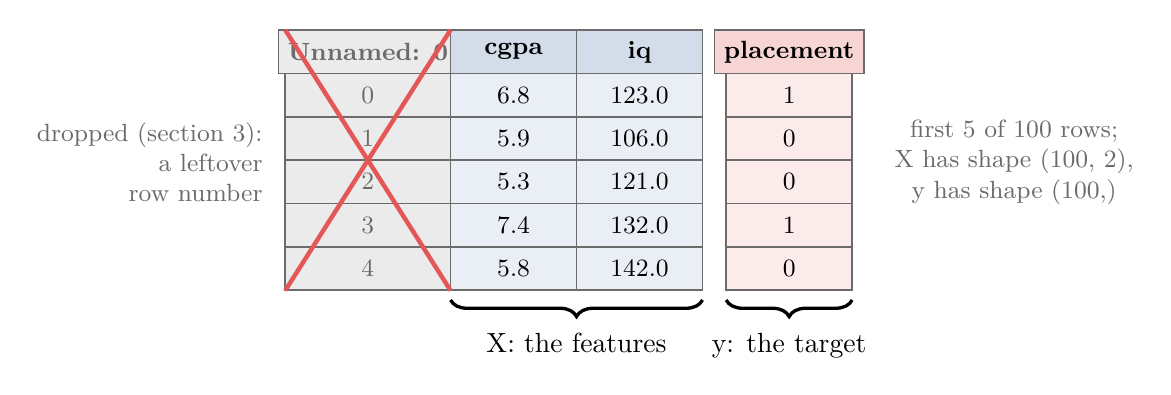
\begin{tikzpicture}[c/.style={draw=cgrey, minimum width=1.6cm, minimum height=0.55cm, font=\sffamily\small, line width=0.6pt},
  hd/.style={c, font=\sffamily\small\bfseries}]
  \foreach \u/\cg/\iq/\p [count=\r] in {0/6.8/123.0/1, 1/5.9/106.0/0, 2/5.3/121.0/0, 3/7.4/132.0/1, 4/5.8/142.0/0} {
    \node[c, fill=black!8, text=cgrey, minimum width=2.1cm] at (-0.25, -0.55*\r) {\u};
    \node[c, fill=cblue!12] at (1.6, -0.55*\r) {\cg};
    \node[c, fill=cblue!12] at (3.2, -0.55*\r) {\iq};
    \node[c, fill=cred!12] at (5.1, -0.55*\r) {\p};
  }
  \node[hd, fill=black!8, text=cgrey, minimum width=2.1cm] at (-0.25, 0) {Unnamed: 0};
  \node[hd, fill=cblue!25] at (1.6, 0) {cgpa}; \node[hd, fill=cblue!25] at (3.2, 0) {iq}; \node[hd, fill=cred!25] at (5.1, 0) {placement};
  \draw[cred, line width=1.6pt] (-1.3, 0.28) -- (0.8, -3.03); \draw[cred, line width=1.6pt] (-1.3, -3.03) -- (0.8, 0.28);
  \node[note, align=right, anchor=east] at (-1.45, -1.4) {dropped (section 3):\\a leftover\\row number};
  \draw[decorate, decoration={brace, amplitude=6pt, mirror}] (0.8, -3.15) -- (4.0, -3.15) node[midway, below=8pt, font=\sffamily] {X: the features};
  \draw[decorate, decoration={brace, amplitude=6pt, mirror}] (4.3, -3.15) -- (5.9, -3.15) node[midway, below=8pt, font=\sffamily] {y: the target};
  \node[note, anchor=west] at (6.3, -1.4) {first 5 of 100 rows;\\X has shape (100, 2),\\y has shape (100,)};
\end{tikzpicture}
\end{document}
